\begin{frame}
  \begin{block}{Algoritmo de Escalonamento de Cargas domésticas baseado em CSA}
    \begin{itemize}
      \item O \textit{Cucko Search Algorithm} (CSA) é um algoritmo
      metaheurístico
      \item ...
    \end{itemize}
  \end{block}
  \begin{figure}[h]
  	\begin{center}
      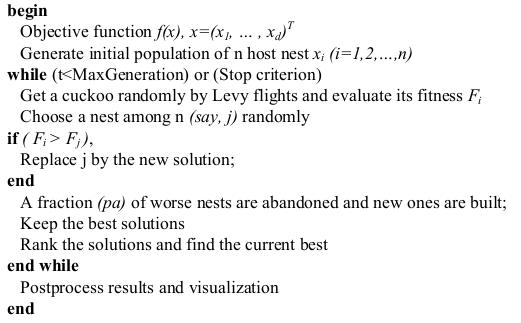
\includegraphics [scale=0.35]{./Figures/csa}
      \caption {Pseudo-código do CSA utilizando vôos de Levy.}
  		%\label{fig:arq-imuno}
  	\end{center}
  \end{figure}
\end{frame}

\begin{frame}
  \begin{block}{}
    \begin{itemize}
      \item Este trabalho é utilizado para determinar o horário de inicio de
      utilização de \alert{utensílios agendáveis}
      \begin{itemize}
        \item Inicialmente obtem-se as preferências dos clientes
        \item Em seguida obtem-se a curva de consumo desejada para a rede
        \item Finalmente o CSA é utilizado para obter-se os horários ótimos de
        inicio de opearação
      \end{itemize}
    \end{itemize}
  \end{block}
  \begin{figure}[h]
  	\begin{center}
      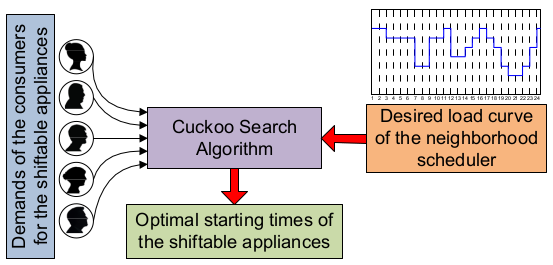
\includegraphics [scale=0.35]{./Figures/CSscheme}
      \caption {Diagrama de blocos da solução proposta.}
  		%\label{fig:arq-imuno}
  	\end{center}
  \end{figure}
\end{frame}

%\begin{frame}
%  \begin{block}{}
%    \begin{itemize}
%      \item
%    \end{itemize}
%  \end{block}
%\end{frame}

%\begin{frame}
%  \begin{block}{}
%  \end{block}
%\end{frame}

%\begin{frame}
%  \begin{figure}[h]
%  	\begin{center}
%      \includegraphics [scale=0.3]{./Figures/Device-Estimates}
%     % \caption {Estimativa de dispositivos conectados à Internet.}
%  		%\label{fig:arq-imuno}
%  	\end{center}
%  \end{figure}
%\end{frame}

%\begin{frame}{Redes de Acesso}
%	\begin{figure}[!htb]
%		\centering
%		\subfloat[DSL]{
%			\includegraphics[height=3.5cm]{./Figures/DSLaccess}
%			\label{figdroopy}}
%		\quad %espaco separador
%		\subfloat[Cable]{
%			\includegraphics[height=3.5cm]{./Figures/CableAccess}
%			\label{figsnoop}}
%		%\caption{Subfiguras}
%		%\label{fig01}
%	\end{figure}
%\end{frame}

%\begin{frame}[fragile]
%\scriptsize
%\begin{verbatim}
%\end{verbatim}
%\end{frame}

%\begin{frame}{\textit{Socket Programming with TCP}}
%\scriptsize
%\lstinputlisting[language=Python, caption={TCP Server.}]{./code/upperServer/TCPserver.py}
%\end{frame}


